% !TEX TS-program = pdflatexmk
\documentclass[12pt]{article}
\usepackage{float}

\usepackage{amsthm}

% Layout.
\usepackage[top=.75in, bottom=0.75in, left=.75in, right=.75in, headheight=1in, headsep=6pt]{geometry}

\usepackage{fancyhdr, enumerate,multirow}
% Fonts.
\usepackage{mathptmx}
\usepackage[scaled=0.86]{helvet}
\renewcommand{\emph}[1]{\textsf{\textbf{#1}}}

% Misc packages.
\usepackage{amsmath,amssymb,latexsym}
\usepackage{graphicx,tikz}
\usepackage{array}
\usepackage{xcolor}
\usepackage{multicol}
\usepackage{tabularx,colortbl}
\usepackage[T1]{fontenc}
\usepackage{enumitem}
%to make tikz pics work
\usepackage{tikz,pgfplots}

\usepackage{varwidth}
\usepackage{verbatim}
\usepackage{mathtools}
\DeclarePairedDelimiter\ceil{\lceil}{\rceil}
\DeclarePairedDelimiter\floor{\lfloor}{\rfloor}

\newenvironment{centerverbatim}{%
  \par
  \centering
  \varwidth{\linewidth}%
  \verbatim
}{%
  \endverbatim
  \endvarwidth
  \par
}

\makeatletter
\newenvironment{centeredverbatim}{\expandafter\verbatim\centering}{\endverbatim}
\makeatother


\usetikzlibrary{arrows}
\newcommand{\midarrow}{\tikz \draw[-triangle 90] (0,0) -- +(.1,0);}

\usepackage[colorlinks=true]{hyperref}

% Paragraph spacing
\parindent 0pt
\parskip 6pt plus 1pt
\def\tableindent{\hskip 0.5 in}
\def\ts{\hskip 1.5 em}

\usepackage{fancyhdr}
\pagestyle{fancy} 
\lhead{\large\sf\textbf{MATH 663 }}
\rhead{\large\sf\textbf{Fall 2023}}
\chead{\large\sf\textbf{HW 8}}

\newcommand{\localhead}[1]{\par\smallskip\textbf{#1}\nobreak\\}%
\def\heading#1{\localhead{\large\emph{#1}}}
\def\subheading#1{\localhead{\emph{#1}}}

%% Special Math Symbol shortcuts
\newcommand{\NN}{\mathbb{N}}
\newcommand{\RR}{\mathbb{R}}

\newcommand{\rad}{\text{rad}}
\newcommand{\diam}{\text{diam}}
\newcommand\solution{\localhead{Solution:}}

%\newenvironment{clist}%
%{\bgroup\parskip 0pt\begin{list}{$\bullet$}{\partopsep 4pt\topsep 0pt\itemsep -2pt}}%
%{\end{list}\egroup}%

\usetikzlibrary{calc,arrows.meta}
%\pgfplotsset{my style/.append style={axis x line=middle, axis y line=
%middle, xlabel={$x$}, ylabel={$y$}, axis equal }}{





\usetikzlibrary{calc,arrows.meta}
%\pgfplotsset{my style/.append style={axis x line=middle, axis y line=
%middle, xlabel={$x$}, ylabel={$y$}, axis equal }}
\usetikzlibrary{arrows}
\newcommand{\marrow}{\tikz \draw[-triangle 90] (0,0) -- +(.1,0);}


\begin{document}
\begin{enumerate}
	\item In the network below, the capacity and flow value for each edge are represented with an ordered pair. Since the flow is everywhere zero, there is no need to direct the edges. However two edges are directed so you can see how to change the diagram.  Find a maximum flow from $s$ to $t$. Prove your answer is optimal by finding a cut with minimum capacity. \\
	
	\begin{center}
		
		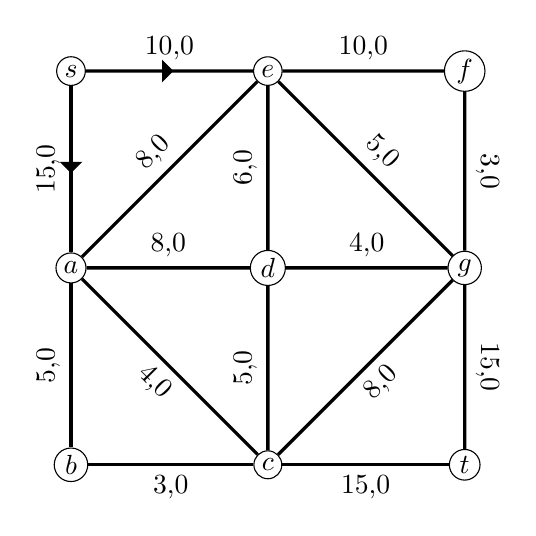
\begin{tikzpicture}[scale=2.5,every node/.style={draw,circle, inner sep=.05 cm}]
			
			\node (s) at (0,2){$s$};
			\node (a) at (0,1){$a$};
			\node (b) at (0,0){$b$};
	\node (c) at (1,0){$c$};
	\node (d) at (1,1){$d$};
	\node (e) at (1,2){$e$};
	\node (f) at (2,2){$f$};
	\node (g) at (2,1){$g$};
	\node (t) at (2,0){$t$};
	\begin{scope}[very thick, every node/.style={sloped,allow upside down}]
	%vertical edges
	\draw (s) -- node{\marrow} node[above,rotate=180]{15,0} (a);
	\draw (a) -- node[above,rotate=180]{5,0} (b);
	\draw (d) -- node[above,rotate=180]{5,0} (c);
	\draw (d) -- node[above]{6,0} (e);
	\draw (f) -- node[above,rotate=0]{3,0} (g);
	\draw (g) -- node[above,rotate=0]{15,0} (t);
	%horizontal edges
	\draw (s) -- node{\marrow} node[above]{10,0} (e);
	\draw (a) -- node[above]{8,0} (d);
	\draw (b) -- node[below]{3,0}  (c);
	\draw (e) -- node[above]{10,0} (f);
	\draw (d) -- node[above]{4,0} (g);
	\draw (c) -- node[below]{15,0}  (t);
	%diagonal edges
	\draw (a) -- node[above]{8,0} (e);
	\draw (a) -- node[below]{4,0}(c);
	\draw (e) -- node[above]{5,0} (g);
	\draw (c) -- node[below]{8,0} (g);
\end{scope}
\end{tikzpicture}
\end{center}
\solution 
First we need to design a feasible flow, then we wil apply the Ford-Fulkerson Algorithm to get the maximal flow, 

\begin{center}
		
	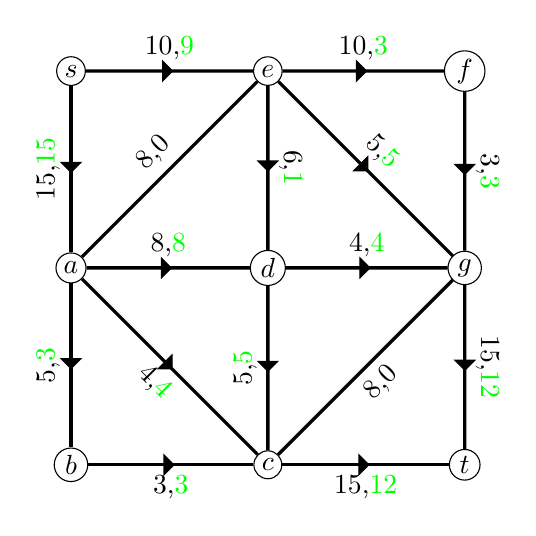
\begin{tikzpicture}[scale=2.5,every node/.style={draw,circle, inner sep=.05 cm}]
		
		\node (s) at (0,2){$s$};
		\node (a) at (0,1){$a$};
		\node (b) at (0,0){$b$};
\node (c) at (1,0){$c$};
\node (d) at (1,1){$d$};
\node (e) at (1,2){$e$};
\node (f) at (2,2){$f$};
\node (g) at (2,1){$g$};
\node (t) at (2,0){$t$};
\begin{scope}[very thick, every node/.style={sloped,allow upside down}]
%vertical edges
\draw (s) -- node{\marrow} node[above,rotate=180]{15,\textcolor{green}{15}} (a);
\draw (a) -- node{\marrow} node[above,rotate=180]{5,\textcolor{green}{3}} (b);
\draw (d) -- node{\marrow}node[above,rotate=180]{5,\textcolor{green}{5}} (c);
\draw (e) -- node{\marrow} node[above]{6,\textcolor{green}{1}} (d);
\draw (f) -- node{\marrow}node[above,rotate=0]{3,\textcolor{green}{3}} (g);
\draw (g) -- node{\marrow} node[above,rotate=0]{15,\textcolor{green}{12}} (t);
%horizontal edges
\draw (s) -- node{\marrow} node[above]{10,\textcolor{green}{9}} (e);
\draw (a) -- node{\marrow} node[above]{8,\textcolor{green}{8}} (d);
\draw (b) -- node{\marrow} node[below]{3,\textcolor{green}{3}}  (c);
\draw (e) -- node{\marrow} node[above]{10,\textcolor{green}{3}} (f);
\draw (d) -- node{\marrow}node[above]{4,\textcolor{green}{4}} (g);
\draw (c) -- node{\marrow}node[below]{15,\textcolor{green}{12}}  (t);
%diagonal edges
\draw (a) -- node[above]{8,0} (e);
\draw (a) -- node{\marrow} node[below]{4,\textcolor{green}{4}}(c);
\draw (e) -- node{\marrow} node[above]{5,\textcolor{green}{5}} (g);
\draw (c) -- node[below]{8,0} (g);
\end{scope}
\end{tikzpicture}
\end{center}
Unfortunately it seems I've discovered the maximal flow, on my first attempt to find a feasible flow. Finding the associated capacity we construct set $S$ from the Ford-Fulkerson algorithm we get $S = \{s, e, f, d, a, b\}$. Note that the cost of the associated cut set $c(S, S^c) = 3 + 5 + 4 + 5 + 4 + 3 = 24$. 




\begin{center}
		
	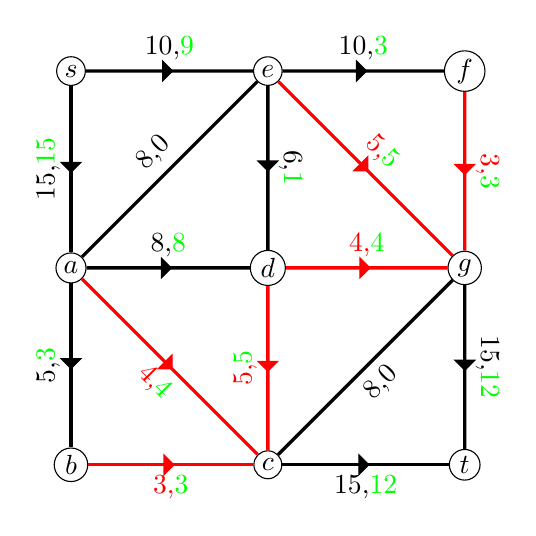
\begin{tikzpicture}[scale=2.5,every node/.style={draw,circle, inner sep=.05 cm}]
		
		\node (s) at (0,2){$s$};
		\node (a) at (0,1){$a$};
		\node (b) at (0,0){$b$};
\node (c) at (1,0){$c$};
\node (d) at (1,1){$d$};
\node (e) at (1,2){$e$};
\node (f) at (2,2){$f$};
\node (g) at (2,1){$g$};
\node (t) at (2,0){$t$};
\begin{scope}[very thick, every node/.style={sloped,allow upside down}]
%vertical edges
\draw (s) -- node{\marrow} node[above,rotate=180]{15,\textcolor{green}{15}} (a);
\draw (a) -- node{\marrow} node[above,rotate=180]{5,\textcolor{green}{3}} (b);
\draw[red] (d) -- node{\marrow}node[above,rotate=180]{5,\textcolor{green}{5}} (c);
\draw (e) -- node{\marrow} node[above]{6,\textcolor{green}{1}} (d);
\draw[red] (f) -- node{\marrow}node[above,rotate=0]{3,\textcolor{green}{3}} (g);
\draw (g) -- node{\marrow} node[above,rotate=0]{15,\textcolor{green}{12}} (t);
%horizontal edges
\draw (s) -- node{\marrow} node[above]{10,\textcolor{green}{9}} (e);
\draw (a) -- node{\marrow} node[above]{8,\textcolor{green}{8}} (d);
\draw[red] (b) -- node{\marrow} node[below]{3,\textcolor{green}{3}}  (c);
\draw (e) -- node{\marrow} node[above]{10,\textcolor{green}{3}} (f);
\draw[red] (d) -- node{\marrow}node[above]{4,\textcolor{green}{4}} (g);
\draw (c) -- node{\marrow}node[below]{15,\textcolor{green}{12}}  (t);
%diagonal edges
\draw (a) -- node[above]{8,0} (e);
\draw[red] (a) -- node{\marrow} node[below]{4,\textcolor{green}{4}}(c);
\draw[red] (e) -- node{\marrow} node[above]{5,\textcolor{green}{5}} (g);
\draw (c) -- node[below]{8,0} (g);
\end{scope}
\end{tikzpicture}
\end{center}


\newpage










	
\item Given $n \in \mathbb{N}$, find a capacity function for the network below such that the algorithm from the proof of the max-flow min-cut theorem (aka Ford-Fulkerson Theorem) will need more than $n$ augmenting paths if the algorithm consistently chooses the path badly.	\\

An \emph{augmenting} path is an $st$-path such that every (directed) edge on the path has available capacity. That is $c(\overrightarrow{e}) > f(\overrightarrow{e}).$ 

\begin{center}
		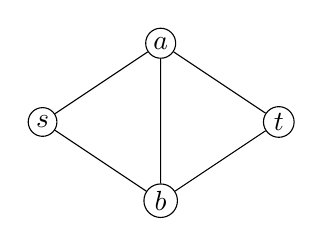
\begin{tikzpicture}[scale=1,every node/.style={draw,circle, inner sep=.05 cm}]
			\node (s) at (0,0){$s$};
			\node (a) at (1.5,1){$a$};
			\node (b) at (1.5,-1){$b$};
			\node (t) at (3,0){$t$};
			\draw (a)--(b)--(s)--(a)--(t)--(b);
		\end{tikzpicture}	
\end{center}


\begin{proof} Consider the following capacity function, 
		\begin{center}
			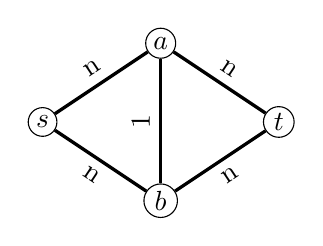
\begin{tikzpicture}[scale=1,every node/.style={draw,circle, inner sep=.05 cm}]
				\node (s) at (0,0){$s$};
				\node (a) at (1.5,1){$a$};
				\node (b) at (1.5,-1){$b$};
				\node (t) at (3,0){$t$};
				\begin{scope}[very thick, every node/.style={sloped,allow upside down}]
				\draw (a)--node[above,rotate=180]{1}(b);
				\draw (b)--node[below,rotate=180]{n}(s);
				\draw (s)--node[above]{n}(a);
				\draw (a)--node[above]{n}(t);
				\draw (t)--node[below,rotate=180]{n}(b);
				\end{scope}
			\end{tikzpicture}	
		\end{center}
		Supposing the FF algorithm consistently chooses the path badly, the edge $ab$ will always be used, alternating direction and only allowing the flow to be increased by 1 unit with each iteration. The algorithm will terminate once both edges $sa$ and $sb$ have flow which saturates their capacities, and hence after $2n$ iterations the FF algorithm will terminate with the following flow,  
		\begin{center}
			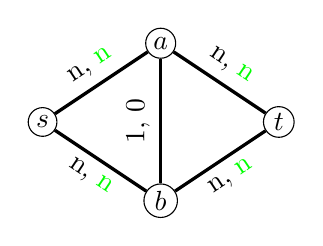
\begin{tikzpicture}[scale=1,every node/.style={draw,circle, inner sep=.05 cm}]
				\node (s) at (0,0){$s$};
				\node (a) at (1.5,1){$a$};
				\node (b) at (1.5,-1){$b$};
				\node (t) at (3,0){$t$};
				\begin{scope}[very thick, every node/.style={sloped,allow upside down}]
				\draw (a)--node[above,rotate=180]{1, 0}(b);
				\draw (b)--node[below,rotate=180]{n, \textcolor{green}{n}}(s);
				\draw (s)--node[above]{n, \textcolor{green}{n}}(a);
				\draw (a)--node[above]{n, \textcolor{green}{n}}(t);
				\draw (t)--node[below,rotate=180]{n, \textcolor{green}{n}}(b);
				\end{scope}
			\end{tikzpicture}	
		\end{center}
	\end{proof}

\newpage


	% Duplicate all vertices non source and sink. 
\item Use the max-flow min-cut theorem to prove part 1 of Corollary 3.3.5. (Copied below.)\\

\begin{quote}
Let $a$ and $b$ be two distinct vertices of the simple graph $G$. If $ab \not \in E$, then the minimum number of vertices separating $a$ from $b$ is equal to the maximum number of independent $ab$-paths in $G.$
\end{quote}
\begin{proof} Let $G$ be a simple graph with distinct vertices $a$ and $b$ such that $ab \not \in E$. Now define a new graph $G'$ such that $V(G') = \left(V(G)\setminus\{a, b\}\right) \sqcup \left(V(G)\setminus\{a, b\}\right) \cup \{a, b\}$ where $v_1$ is from the first copy of $V(G)\setminus\{a, b\}$ and $v_2$ from the second. Now define $E(G')$ by the following, 
	\begin{center}
		$v_1v_2 \in E(G')$ if $v \in V(G)\setminus\{a, b\}$, \\
		$u_1v_2, u_2v_1 \in E(G')$ if $uv \in V(G)\setminus\{a, b\}$,\\ 
		$av_1 \in E(G')$ if $av \in E(G)$ and, $v_2b \in E(G')$ if $vb \in E(G)$. 
	\end{center}

	Now we define the following capacity function, 
	\begin{equation*}
		c(e) = \begin{cases}
			1, & e = v_1v_2,\\
			\infty, & e = v_2u_1, \quad e= av_1, \quad e = v_2b\\
			0& \text{otherwise}.
		\end{cases}
	\end{equation*}

So we define a network $N = (G', a, b, c)$. Now consider a flow $f$ on $N$ such that $f$ is maximum, and the corresponding cut $S$. By Ford-Fulkerson we know that $|f| = c(S, \overline{S})$. We aim to show that we, have constructed $N$ is such a way that $|f|$ is the maximum number of independent $ab$ paths in $G$ and $|S|$ is the minimum number of vertices separating $a$ and $b$. 

We will first argue that $|f|$ is the maximum number of independent $ab$ paths in $G$.
Start with a zero flow, the FF algorithm will increment the flow by 1 after each iteration by how we have constructed our capacity function (flow must traverse a $v_1v_2$ edge).

Now let $P$ and $P'$ be $ab$-paths from different iterations of the FF algorithm, where $P$ came before $P'$. Suppose for the sake of contradiction that they share a vertex. The vertex is either a $v_1$ or a $v_2$ vertex. Suppose it is a $v_1$ vertex, then $v_1v_2 \in P, P'$ but since $P$ and $P'$ are different iterations of the FF algorithm, this must be a contradiction as $v_1v_2$ would already have a saturated capacity after $P$. Now suppose a $v_2$ vertex is shared, well by the construction of our capacity function $v_1$ must also be shared, and again we have a contradiction. Since each iteration of the FF algorithm identifies an independent path we can conclude that $|f|$ is the maximum number of independent $ab$ paths in $G$


It seems as though $S$ cannot contain a non $v_1v_2$ edge, as that would imply the flow through such an edge meets the capacity, which is infinity. Therefore $S$ only contains edges that correspond to vertices in $G$ and by construction $|S|$ is the minimum number of vertices separating $a$ and $b$. 
\end{proof}
\newpage


\item Determine the value of $ex(n,K_{1,r})$ for all $r$ and $n$. (Assume that $n>r.$)
\begin{proof} Rephrasing $ex(n,K_{1,r})$, what is the maximum number of edges in an $n$ vertex graph, such that no vertex is degree $r$ or higher. If no vertex is degree $r$, then to maximize the number of edges, all vertices must have degree $r - 1$. Applying the handshake lemma to count the number of edges and applying the floor function to deal with the parity of $n$ we get that, 
	\begin{equation*}
		ex(n,K_{1,r}) = \floor{\frac{n(r - 1)}{2}}.
	\end{equation*}
\end{proof}
\newpage


\item Show that every connected graph $G$, on at least three vertices contains a path or a cycle of length at least $\min\{2\delta, |G|\}.$
\begin{proof} Let $G$ be a graph such that $|G| \geq 3$, and suppose for the sake of contradiction that every path and cycle of $G$ has length strictly less than $\min\{2\delta, |G|\}.$ Let $x_1Px_k$ be a maximum path on $k$ vertices, with length $k - 1$. Note $x_1x_k \not\in E(G)$ otherwise $P$ would form a cycle of length $k < |G|$, and since $G$ is connected a longer path $P'$ could be formed with vertex $v' \not\in P$ through $x_1x_k$. Now for every $v_i \in P$, that is also $v_i \in N(v_1)$ it must be the case that $v_{i - 1} \not\in N(v_k)$ otherwise $v_iv_1Pv_{i - 1}v_k$ would be a longer path. Note that $v_1$ has at least $\delta$ neighbors among the set of $k - 1$ possible neighbors in $P$, which leaves only $k - 1 - \delta$ neighbors for $v_k$ however since $k - 1 - \delta < \delta$ by our hypothesis we have a contradiction.
	
	


\end{proof}
\newpage


% By 5 we are garuneteed a bertex of minimum degree that is small to prevent a path or cycle by 5
\item Prove the Erd\"{o}s-S\"os Conjecture for the case when the tree is a path. (Hint: use the previous problem.)
\begin{proof} Recall the Erd\"{o}s-S\"os Conjecture which states that $ex(n, T) \leq \frac{1}{2}(k - 1)n$ for all trees with $k \geq 2$ edges; for all $n$ this is the best possible bound for every tree $T$. \\

	Suppose $T$ is a path, with length $k \geq 2$, and for the sake of contradiction assume $ex(n, T) > \frac{1}{2}(k - 1)n$, so there exists a graph $G$ on $n$ vertices with no length $k$ paths and $||G|| > \frac{1}{2}(k - 1)n$. Note that $||G|| = \frac{1}{2}d(G)n > \frac{1}{2}(k - 1)n$ which implies that $e(G) = \frac{1}{2}d(G) > \frac{1}{2}(k - 1)$. Since $G$ is a graph with at least one edge, there exists a subgraph $H$, such that $\delta(H) \geq e(G)$(Prop 1.2.2). Now it follows that,
	\begin{align*}
		\delta(H) \geq e(G) &> \frac{1}{2}(k - 1),\\
		2\delta(H) &> (k - 1),\\
		2\delta(H) &\geq k.
	\end{align*}
	Therefore by problem 5 we know that $H$ contains a path of length at least $k$, and since $H$ is a subgraph of $G$ it follows that $G$ contains that path as well, a contradiction.
	








\end{proof}
\end{enumerate}
\end{document}